% Diagrama de Classes
\section{Diagrama de Classes}

\label{pro:classes}

\begin{figure}[!htp]
  \begin{center}
    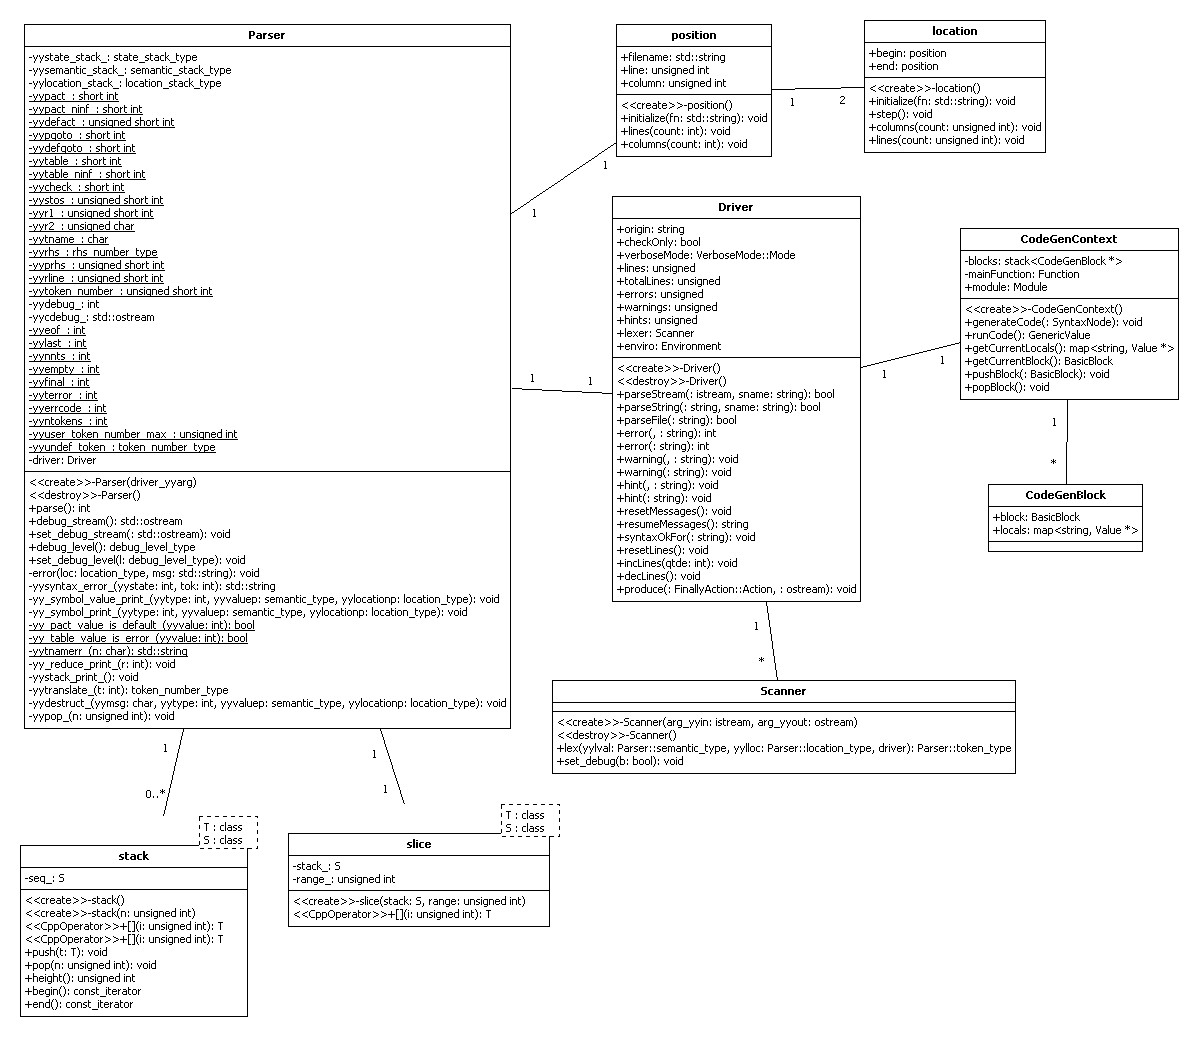
\includegraphics[width=1\textwidth]{figuras/classes1}
  \end{center}
  \caption{Classes principais de manipula\ca o dos programas}
  \label{fig:classes1}
\end{figure}

A classe\footnote{N.A. O diagrama de classes necessitou ser dividido em algumas partes, pois se todas as classes ficassem juntas, seria imposs\ih vel l\^e-las.} \emph{Parser} \eh\ gerada automaticamente pelo programa \emph{Bison}\ref{pro:bison} e a classe \emph{Scanner} \eh\ gerada pelo programa \emph{Flex}\ref{pro:flex}.

A classes \emph{CodeGenBlock} e \emph{CodeGenContext} fazem uso das classes presentes no projeto LLVM\footnote{N\ao\ constar\ao\ aqui as classes do projeto LLVM, pois n\ao\ \eh\ o objetivo do projeto explicar detalhes de sua constru\ca o.}.

A classe \emph{Driver} direciona o funcionamento do sistema, interpretando as flags fornecidas via linha de comando.

\begin{figure}[!htp]
  \begin{center}
    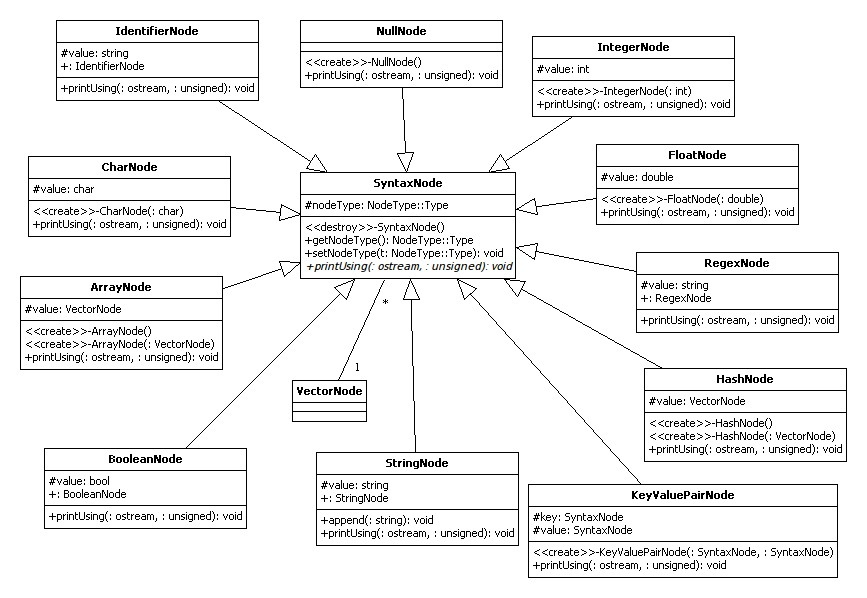
\includegraphics[width=1\textwidth]{figuras/classes2}
  \end{center}
  \caption{Classes que representam os valores primitivos da linguagem}
  \label{fig:classes2}
\end{figure}

\begin{figure}[!htp]
  \begin{center}
    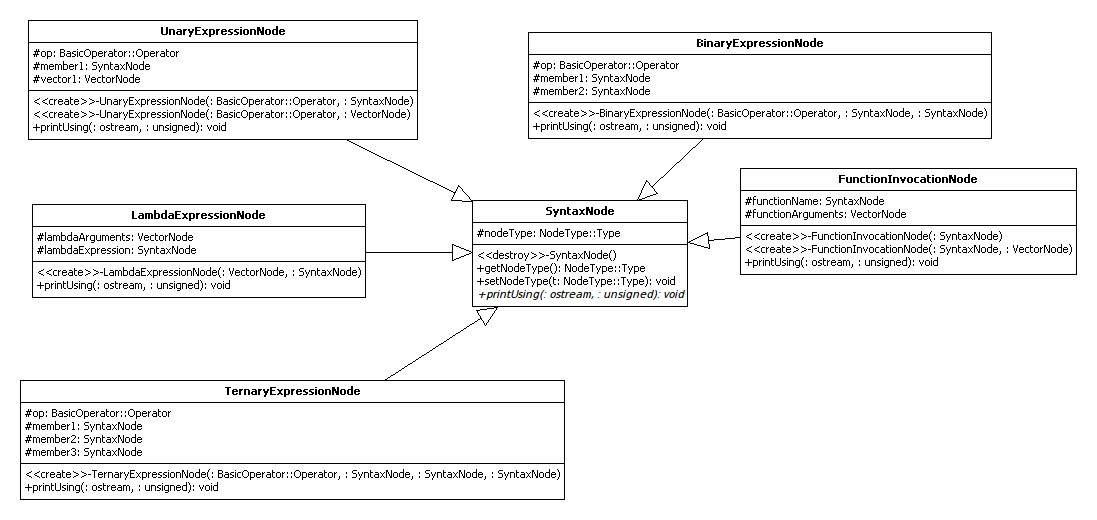
\includegraphics[width=1\textwidth]{figuras/classes3}
  \end{center}
  \caption{Classes que representam as express\~oes da linguagem}
  \label{fig:classes3}
\end{figure}

\begin{figure}[!htp]
  \begin{center}
    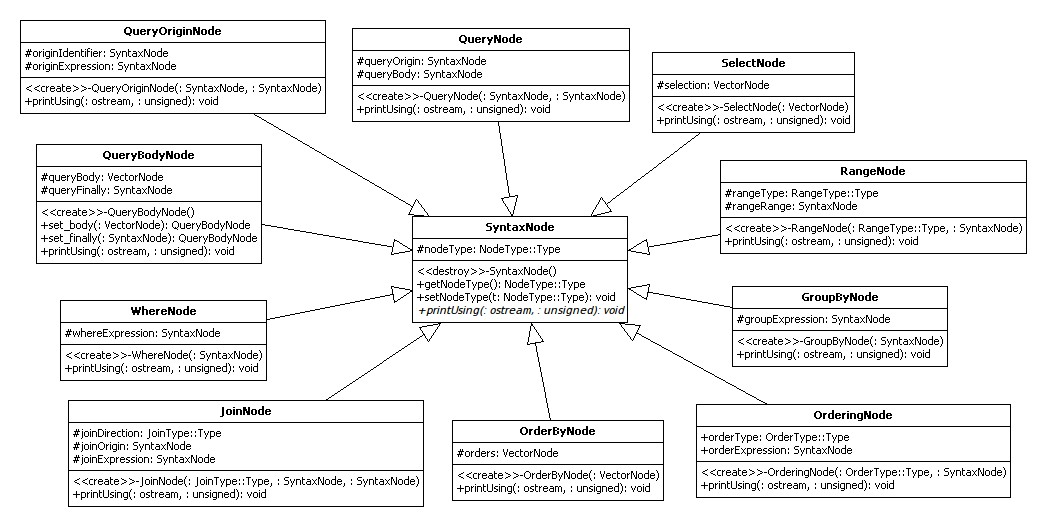
\includegraphics[width=1\textwidth]{figuras/classes4}
  \end{center}
  \caption{Classes que representam as express\~oes de consulta da linguagem}
  \label{fig:classes4}
\end{figure}

\begin{figure}[!htp]
  \begin{center}
    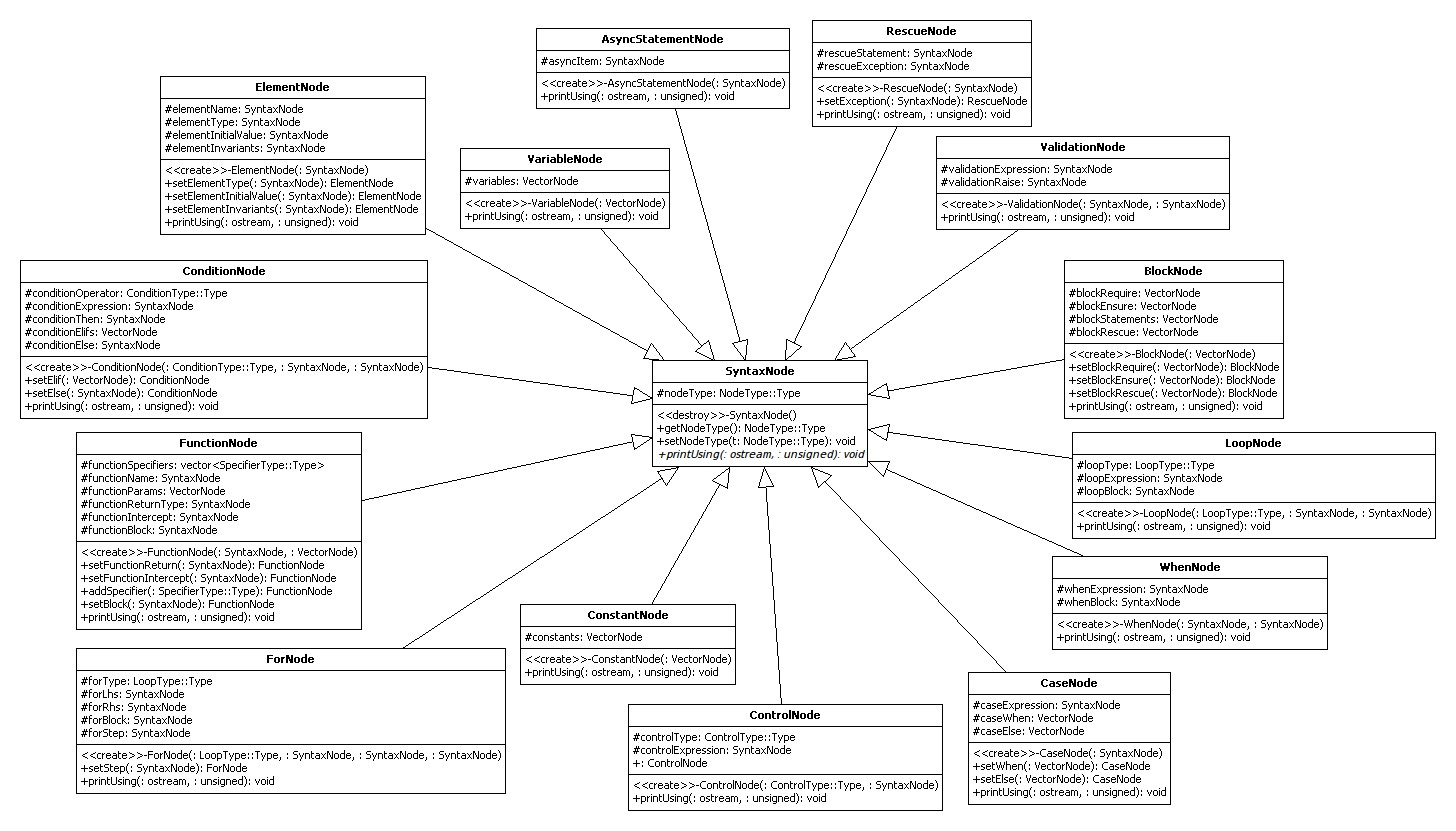
\includegraphics[width=1\textwidth]{figuras/classes5}
  \end{center}
  \caption{Classes que representam as estruturas de comando e controle da linguagem}
  \label{fig:classes5}
\end{figure}

\begin{figure}[!htp]
  \begin{center}
    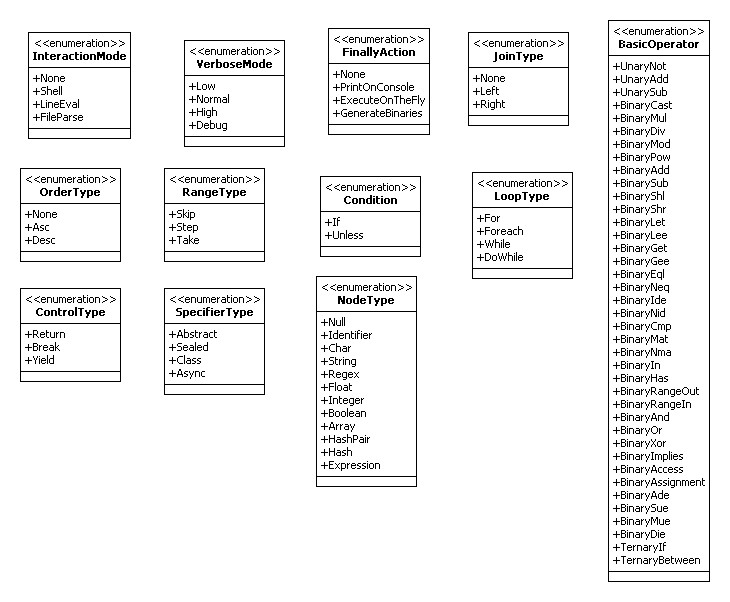
\includegraphics[width=1\textwidth]{figuras/classes6}
  \end{center}
  \caption{Enumera\co es que auxiliam o tratamento das constru\co es da linguagem}
  \label{fig:classes6}
\end{figure}
